\documentclass[../main.tex]{subfiles}

\begin{document}
\chapter{Folgen und Reihen}
\section{Folgen}
\begin{definition}
	Eine \emph{Folge} in $\mathbb{R}$ ist eine Abbildung
  \begin{align*}
    a \colon \mathbb{N} & \to \mathbb{R} \\
    n & \mapsto a_n.
  \end{align*}
  Wir notieren das häufig als 
  $(a_0, a_1, a_2, \dots) = {(a_n)}_{n \in \mathbb{N}}$.
	Eine Folge ${(a_n)}_{n \in \mathbb{N}}$ in $\mathbb{R}$
	heisst \emph{konvergent} mit Grenzwert
	$L \in \mathbb{R}$, falls für alle
	$\varepsilon \in \mathbb{R}$ mit $\varepsilon > 0$
	eine Zahl $N \in \mathbb{N}$ existiert,
	so dass für alle $n\in \mathbb{N}$ 
	mit $n \geq N$ gilt, dass
	$|a_n - L| \leq \varepsilon$. In diesem Fall schreiben wir
	\[
	  \lim_{n \to \infty} a_n = L.
	\]
\end{definition}

In anderen Worten bedeutet $\lim_{n \to \infty} a_n = L$, dass
für vorgegebenes $\varepsilon > 0$
ab einem gewissen Index die Folge für immer im Intervall
$[L- \varepsilon, L + \varepsilon]$ liegt.

\begin{examples}
  \leavevmode
\begin{enumerate}[(1)]
  \item Sei $a_n = 1/n$ für $n \geq 1$. Wir behaupten,
	  dass diese Folge konvergent mit Grenzwert
	  $0 \in \mathbb{R}$ ist. Dazu sei $\varepsilon > 0$
	  vorgegeben.
	  Nach dem Archimedischen Prinzip
	  existiert $N \in \mathbb{N}$ mit
	  $N > 1/\varepsilon$.
	  Dann gilt für alle $n \in \mathbb{N}$ mit $n \geq N$,
	  dass $n > 1/\varepsilon$, also insbesondere
	  nach dem zweiten Ordnungsaxiom, dass
	  $1/n < \varepsilon$.
	  Folglich ist
	  \[
		  |a_n - 0| = \frac{1}{n} < \varepsilon,
	  \]
	  also
	  \(
		  \lim_{n \to \infty}\frac{1}{n} = 0.
	  \)
	  Varianten davon sind
	  \begin{itemize}
	    \item $\lim_{n \to \infty} \frac{1}{n^2} = 0$,
	    \item $\lim_{n \to \infty} \frac{1}{\sqrt n} = 0$,
	    \item $\lim_{n \to \infty} \frac{1}{n^a} = 0$ für
		    eine ``vernünftige'' Potenz $a$.
	  \end{itemize}
  \item Sei $a_n = \sqrt[n]{n}$. Wir behaupten, dass
	  \[
		  \lim_{n \to \infty} \sqrt[n]{n} = 1.
	  \]
	  Wir wollen zeigen, dass 
	  \[
		  \sqrt[n]{n} \leq 1 + \sqrt{\frac{2}{n-1}}.
	  \]
	  Tatsächlich gilt
	  \[
		  n  \leq {\left( 1 + \sqrt{\frac{2}{n-1}} \right)}^n,
	  \]
	  denn Anwenden der binomischen Formel
	  \[
		  {(a + b)}^n = \binom{n}{0}a^n + \binom{n}{1}a^{n-1}b
		  + \cdots + \binom{n}{n-1}ab^{n-1} + \binom{n}{n}b^n
	  \]
	  liefert
	  \[
		  {\left( 1 + \sqrt{\frac{2}{n-1}} \right)}^n
		  = 1 + n \cdot \sqrt{\frac{2}{n-1}}
		  + \binom{n}{2} {\left( \sqrt{\frac{2}{n-1}} \right)}^2
		  + R
	  \]
	  mit $R \geq 0$.
    Wir interessieren uns nur für den 
    quadratischen Term.
    Bemerke, dass
    \[
      \binom{n}{2}{\left( \sqrt{\frac{2}{n-1}} \right)}^2
      = \frac{n(n-1)}{2} \frac{2}{n-1} = n.
    \]
	  Somit gilt für alle $n \geq 1$ die Ungleichung
	  \[
		  1 \leq \sqrt[n]{n} \leq 1 + \sqrt{\frac{2}{n-1}}.
	  \]
	  Aus
	  \[
		  \lim_{n \to \infty} 1 + \sqrt{\frac{2}{n-1}} = 1,
	  \]
    was eine Variation vom ersten Beispiel ist, folgt nun auch
	  \[
		  \lim_{n \to \infty} \sqrt[n]{n} = 1.
	  \]
  \item Sei $q \in \mathbb{R}$ mit $q \geq 0$. Dann gilt
	  \[
	    \lim_{n \to \infty} q^n = 
	    \begin{cases}
		    0, & \text{falls } q < 1, \\
		    1, & \text{falls } q = 1, \\
		    +\infty, & \text{falls } q > 1.
	    \end{cases}
	  \]
	Die Notation
	\(
	  \lim_{n \to \infty} a_n = + \infty
	\)
	heisst, dass für alle $S > 0$ ein Index $N \in \mathbb{N}$
	existiert, so dass für alle $n \geq N$ gilt, dass
	$a_n > S$ ist.
	Der zweite der Fälle ist klar. Für den dritten Fall, 
	betrachte
	\[
		q^n = {\left( 1 + (q-1) \right)}^n \geq 1 + n(q-1),
	\]
	wobei $q-1 > 0$. 
	Sei $S > 0$ vorgegeben. Wähle $N \in \mathbb{N}$ mit
	\(
  N \geq {S}/{(q-1)}.
	\)
	Für alle $n \geq N$ gilt dann $q^n \geq 1 + S > S$.
	Für den ersten Fall ersetze $q$ durch $1/q$.
\end{enumerate}
\end{examples}

\section{Cauchyfolgen}
\begin{definition}
Eine Folge 
${\left( a_n \right)}_{n \in \mathbb{N}}$ in $\mathbb{R}$ 
heisst \emph{Cauchyfolge}, so dass für alle
vorgegebenen $\varepsilon > 0$ ein $N \in \mathbb{N}$ existiert,
so dass für alle $n, m \in \mathbb{N}$ mit $n,m \geq N$ gilt,
dass $|a_n - a_m| \leq \varepsilon$.
\end{definition}

In anderen Worten, ab einem gewissen Index sind alle
Folgenglieder höchstens $\varepsilon$ voneinander 
entfernt. Die Definition der Konvergenz unterscheidet
sich dadurch, dass bei Cauchyfolgen kein Grenzwert
erwähnt wird: nur Folgeglieder werden verglichen.

\begin{theorem}[Konvergenzprinzip
  von Cauchy, 1789--1857]
Für Folgen ${\left( a_n \right)}_{n \in \mathbb{N}}$ in $\mathbb{R}$
  sind äquivalent:
  \begin{enumerate}[\normalfont(i)]
    \item Die Folge ${\left( a_n \right)}_{n \in \mathbb{N}}$
      ist konvergent.
    \item Die Folge ${\left( a_n \right)}_{n \in \mathbb{N}}$
      ist eine Cauchyfolge.
  \end{enumerate}
\end{theorem}

\begin{proof}
  Die Implikation (i) $\Rightarrow$ (ii) ist eine Übung.
  Dazu kann  
  \[
    |a_n - a_m| \leq |a_n - L| + |L - a_m|
  \]
  verwendet werden. Diese Ungleichung wird auch
  \emph{Dreiecksungleichung} genannt (das Dreieck
  ist hier degeneriert, das heisst es liegt
  auf einer Linie, und die Eckpunkte sind
  $a_n, a_m$ und $L$).

  Die Umkehrung (ii) $\Rightarrow$ (i) ist etwas schwieriger.
Sei ${\left( a_n \right)}_{n \in \mathbb{N}}$ eine
  Cauchyfolge.
  Betrachte für alle $k \in \mathbb{N}$ die Menge
  \[
    A_k = \left\{ a_{k}, a_{k+1}, \dots \right\}
    \subset \mathbb{R}.
  \]
  Wir behaupten, dass diese Mengen $A_k$
  (von oben und unten)
  beschränkt sind.
  Zum Beweis betrachte $\varepsilon = 1 > 0$.
  Dann existiert ein $N \in \mathbb{N}$ mit
  der Eigenschaft, dass immer wenn
  $n, m \geq N$, dann folgt
  $|a_n - a_m| \leq 1$.
  Setze
  \[
  S_k = \max \{|a_k|, |a_{k+1}|, \dots, |a_{N-1}|, |a_N| + 1\}.
  \]
  Dann gilt für alle $n \geq k$, dass $|a_k| \leq S_k$.
  Tatsächlich ist für $n \geq N$ die Ungleichung
  $|a_n - a_N| \leq \varepsilon = 1$
  erfüllt, also folgt $|a_n| \leq |a_N| + 1$.
  Analog existiert eine untere Schranke $I_k$ für 
  $A_k$.
  Dies zeigt die Behauptung.

  Nun gilt für alle $k \in \mathbb{N}$, dass
  $I_k \leq A_k \leq S_k$ (wobei $A_k \subset \mathbb{R}$
  und $I_k, S_k \in \mathbb{R}$).
  Wende die Vollständigkeit von $\mathbb{R}$ 
  auf die beiden Teilmengen
  $\left\{ I_0, I_1, \dots \right\} $
  und $\{S_0, S_1, \dots\}$ an: Es existiert
  $L \in \mathbb{R}$, so dass für alle
  $k \in \mathbb{N}$ gilt, dass $I_k \leq L \leq S_k$.

  Wir behaupten nun, dass
  \[
    \lim_{n \to \infty} a_n = L.
  \]
  Um das zu beweisen, müssen wir die formale
  Definition der Konvergenz anwenden.
  Sei also $\varepsilon > 0$ vorgegeben.
  Dann existiert $N \in \mathbb{N}$ 
  so dass immer wenn $n, m \geq N$, dann auch
  $|a_n - a_m| \leq \varepsilon$,
  da ${(a_n)}_{n \in \mathbb{N}}$ eine Cauchyfolge ist.
  Daraus folgt, dass
  \[
    |\sup A_N - \inf A_N| \leq \varepsilon,
  \]
  da die nicht-strikte Ungleichung für alle
  Elemente von $A_N$ gilt.
  Nach Konstruktion gilt $\inf A_N \leq L \leq \sup A_N$.
  Ausserdem gilt für alle $n \geq N$, dass
  \[
    |a_n - L| \leq |S_N - I_N| \leq \varepsilon,
  \]
  da $I_N \leq a_n \leq S_N$.
\end{proof}

Zusammengefasst haben wir die Folgeglieder
erst ab einem späten Index betrachtet und
unter Verwendung der Vollständigkeit
gezeigt, dass wir einen Grenzwert $L$
finden können.

\begin{remark}
  In geordneten Körpern,
  die das archimedische Prinzip erfüllen,
  sind folgende Prinzipien äquivalent.
  \begin{itemize}
    \item Vollständigkeit,
    \item das Supremumsprinzip,
    \item das Konvergenzprinzip von Cauchy.
  \end{itemize}
  
\end{remark}


Die Beobachtung, dass die Folge $I_0, I_1, I_2, \dots$
im Beweis oben konvergiert, lässt sich verallgemeinern.
Eine Folge ${(a_{n})}_{n \in \mathbb{N}}$ 
so dass für alle $n \in \mathbb{N}$ gilt,
dass $a_n \leq a_{n+1}$, heisst \emph{monoton wachsend}.

\begin{monotony}
  Sei ${(a_n)}_{n \in \mathbb{N}}$ eine monoton wachsende
  Folge in $\mathbb{R}$,
  welche nach oben beschränkt ist.
  Dann konvergiert ${(a_n)}_{n \in \mathbb{N}}$ mit
  Grenzwert
  \(
    S = \sup \{a_0, a_1, a_2, \dots\}.
  \)
\end{monotony}

\begin{proof}
  Da $\{a_0, a_1, a_2, \dots\}$ nach oben beschränkt ist,
  ist $S \in \mathbb{R}$ definiert und eine reelle Zahl.
  Wir zeigen nun, dass
  \[
    \lim_{n \to \infty} a_n = S
  \]
  gilt.
  Sei dazu $\varepsilon > 0$ vorgegeben. 
  Dann ist $S - \varepsilon$ keine obere Schranke
  für $\{a_0, a_1, a_2, \dots\}$,
  da $S$ die kleinste obere Schranke ist.
  Also existiert $N \in \mathbb{N}$ mit
  $a_N > S - \varepsilon$.
  Dann gilt für alle $n \geq N$, dass
  \[
    S - \varepsilon < a_N \leq a_n \leq S,
  \]
  also $|a_n - S| \leq \varepsilon$.
\end{proof}

\begin{example}
  Betrachte die Folge ${(a_n)}_{n \in \mathbb{N}}$ 
  gegeben durch
   \[
   a_n = {\left( 1 + \frac{1}{n} \right)}^n.
   \]
   Es gilt $a_1 = 2$, $a_2 = 9/4$, $a_3 = 64/27, \dots$.
   Wir behaupten, dass
   \begin{enumerate}[(i)]
     \item ${(a_n)}_{n \in \mathbb{N}}$ monoton wachsend ist,
     \item für alle $n \in \mathbb{N}$ gilt, dass
       $a_n \leq 3$.
   \end{enumerate}
   Der Beweis dieser Behauptung ist eine Übung auf
   der Serie 4. Hier machen wir deshalb nur eine Beweisskizze:
   \begin{enumerate}[(i)]
     \item Es kann gezeigt werden, dass
       \[
         {\left( 1 + \frac{1}{n} \right) }^n \leq
         {\left( 1 + \frac{1}{n+1} \right)}^{n+1},
       \]
       indem 
       \[
         {\left( 1 - \frac{1}{{(n+1)}^2} \right)}^n =
         {\left( \frac{1 + \frac{1}{n+1}}{1 + \frac{1}{n}} \right) }
         \geq \frac{1}{1 + \frac{1}{n+1}}
                       = 1 - \frac{1}{n+2}
       \]
       berechnet wird.
     \item
       Die Ungleichung ${(1 + 1/n)}^n \leq 3$ ist äquivalent
       zur Ungleichung ${(n + 1)}^n \leq 3n^n$.
       Man kann dann zeigen, dass
       \[
         {(n+1)}^n =
         \sum_{k=0}^{n} \binom{n}{k}n^k 
         \leq \left( 1 + \frac{1}{1!}
         + \frac{1}{2!} + \frac{1}{3!} + \cdots +
       \frac{1}{n!}\right) \cdot n^n.
       \]
   \end{enumerate}
\end{example}

\begin{remark}
  Der Grenzwert der Folge oben ist
  \[
    \lim_{n \to \infty} {\left( 1 + \frac{1}{n} \right)}^n = e,
  \]
  die \emph{Eulersche Zahl} (die wir noch nicht definiert haben).
\end{remark}

\subsection*{Teilfolgen}
Wir bemerken, dass
\begin{enumerate}[(i)]
  \item jede konvergente Folge beschränkt ist,
  \item es beschränkte Folgen gibt, welche nicht konvergieren,
    zum Beispiel $a_n = {(-1)}^n$.
\end{enumerate}

\begin{definition}
  Sei ${(a_n)}_{n \in \mathbb{N}}$ eine Folge in $\mathbb{R}$ 
  und ${(n_k)}_{k \in \mathbb{N}}$ eine Folge in $\mathbb{N}$,
  welche streng monoton wachsend ist, das heisst
  \(
    n_0 < n_1 < n_2 < \cdots.
  \)
  Dann heisst die Folge ${(a_{n_k})}_{k \in \mathbb{N}}$ 
eine \emph{Teilfolge} von ${(a_n)}_{n \in \mathbb{N}}$.
\end{definition}

In anderen Worten ist eine Teilfolge einer Folge
die Folge die man erhält, wenn man Folgeglieder
wegnimmt, so dass aber noch unendlich viele
Folgeglieder übrigbleibt.

\begin{theorem}[Bolzano-Weierstrass]\label{thm:bolzano-weierstrass}
  Sei ${(a_n)}_{n \in \mathbb{N}}$ eine Folge in $\mathbb{R}$,
  welche von oben und unten beschränkt ist.
  Dann hat die Folge ${(a_n)}_{n \in \mathbb{N}}$
  eine konvergente Teilfolge.
\end{theorem}

\begin{example}
  Die Folge ${(a_n)}_{n \in \mathbb{N}}$ mit Folgegliedern
  $a_n = {(-1)}^n$ hat zwei naheliegende konvergente Teilfolgen,
  nämlich ${(a_{2k})}_{k \in \mathbb{N}}$ mit Grenzwert $1$,
  und ${(a_{2k+1})}_{k \in \mathbb{N}}$ mit Grenzwert $-1$.
  Es gibt aber noch mehr Folgen von Indizes 
  ${(n_k)}_{k \in \mathbb{N}}$, die
  konvergente Teilfolgen liefern.
\end{example}

\begin{proof}[Beweis von Theorem~\ref{thm:bolzano-weierstrass}]
  Sei ${(a_n)}_{n \in \mathbb{N}}$ beschränkt, das heisst
  es existieren $x, y \in \mathbb{R}$, so dass für
  alle $n \in \mathbb{N}$ gilt, dass $x \leq a_k \leq y$.
  Wir unterscheiden nun zwei Fälle.
  \begin{enumerate}[1.]
    \item Die Menge $\{a_0, a_1, a_2, \dots\}$ ist endlich.
      Dann hat die Folge ${(a_n)}_{n \in \mathbb{N}}$ 
      eine konstante Teilfolge
      ${(a_{n_k})}_{k \in \mathbb{N}}$.
      Diese ist konvergent.
    \item Die Menge $\{a_0, a_1, a_2, \dots\}$ ist unendlich.
      Wir konstruieren eine sogenannte Intervallschachtelung.
      Setze 
      \(
        I_0 = [x, y] = \left\{z \in \mathbb{R} 
        \mid x \leq z \leq y\right\}.
      \)
      Wähle $a_{n_0} = a_0 \in I_0$. Halbiere $I_0$, also
      schreibe
      \[
        I_0 = \left[ x, \frac{x+y}{2} \right] 
        \cup \left[ \frac{x+y}{2}, y \right].
      \]
      Eines dieser beiden Teilintervalle enthält
      unendlich viele Folgeglieder,
      das heisst Elemente der Menge
      $\{a_0, a_1, a_2, \dots\}$. Nenne dieses Intervall
      $I_1 = [x_1, y_1]$. Wähle $a_{n_1} \in I_1$
      mit $n_1 > n_0$. Das können wir fordern,
      da es unendlich viele Folgeglieder in 
      $I_1$ gibt.
      Halbiere wie oben $I_1$ und schreibe
      \[
        I_1 = \left[ x_1, \frac{x_1 + y_1}{2} \right] 
        \cup \left[ \frac{x_1 + y_1}{2}, y_1 \right].
      \]
      Wieder enthält eines dieser Intervalle
      unendlich viele Folgeglieder. Nenne dieses
      Intervall $I_2 = [x_2, y_2]$. Wähle
      $a_{n_2} \in I_2$ mit $n_{2} > n_1$.
      Iteriere dieses Verfahren und erhalte eine
      Teilfolge $a_{n_0}, a_{n_1}, a_{n_2}, \dots$.

      Wir behaupten, dass ${(a_{n_k})}_{k \in \mathbb{N}}$
      eine Cauchyfolge (und deshalb konvergent) ist.
      Zum Beweis berechnen wir die Breite des
      Intervalls $I_k$. Berechne
      \[
        y_k - x_k = \frac{y - x}{2^k}.
      \]
      Sei $\varepsilon > 0$ vorgegeben. Wähle
      $N \in \mathbb{N}$ so, dass
      \(
        (y-x)/{2^N} \leq \varepsilon.
      \)
      Dann gilt für alle $k, \ell \geq N$, dass
      $a_{n_k}, a_{n_\ell} \in I_N$ höchstens
      $\varepsilon$ voneinander entfernt sind.
      Konkreter,
      \[
        |a_{n_k} - a_{n_\ell}| 
        \leq \frac{y-x}{2^N} \leq \varepsilon. \qedhere
      \]
  \end{enumerate}
\end{proof}

\begin{definition}
  Eine Zahl $\alpha \in \mathbb{R}$ heisst
  \emph{Häufungspunkt} einer Folge
  ${(a_{n})}_{n \in \mathbb{N}}$ in $\mathbb{R}$,
  falls es eine konvergente Folge
  ${(a_{n_k})}_{k \in \mathbb{N}}$ gibt
  mit
  \[
    \lim_{k \to \infty} a_{n_k} = \alpha.
  \]
\end{definition}

\begin{examples}
  \leavevmode
  \begin{enumerate}[(i)]
    \item Bei der Folge $a_n = (-1)^n$ ist die Menge
      der Häufungspunkte $\{-1, 1\}$.
    \item Sei $a \colon \mathbb{N} \to \mathbb{Q}$ eine
      beliebige
      Bijektion. Dann ist jede reelle Zahl ein Häufungspunkt,
      das heisst die Menge der Häufungspunkte
      ist $\mathbb{R}$. Das ist erstaunlich, da abzählbar
      viele Folgeglieder überabzählbar viele
      Häufungspunkte hervorrufen. Zum Beweis,
      dass tatsächlich jede reelle Zahl ein Häufungspunkt
      ist, sei $\alpha \in \mathbb{R}$. Wähle
      $n_0 \in \mathbb{N}$ mit $|\alpha - a_{n_0}| \leq 1$.
      Wähle dann $n_{1} > n_0$ mit $|\alpha - a_{n_1}| \leq 1/2$.
      Wähle iterativ $n_{k} > n_{k-1}$ mit $|\alpha - a_{n_k}|
      \leq 1/2^k$. Dies ist möglich, da jedes Intervall der
      Form
      $[\alpha - 1/2^k, \alpha + 1/2^k]$ unendlich viele
      rationale Zahlen enthält. Wir können auch $n_k > n_{k-1}$
      einrichten, da bei der $k$-ten Wahl erst endlich viele
      rationale Zahlen bereits belegt sind.
      Es gilt also
      \(
        \lim_{k \to \infty} a_{n_k} = \alpha.
      \)
  \end{enumerate}
\end{examples}


\subsection*{Rechenregeln}
\begin{proposition}
  Seien ${(a_n)}_{n \in \mathbb{N}}$ und
  ${(b_n)}_{n \in \mathbb{N}}$ zwei
  konvergente Folgen in $\mathbb{R}$ mit Grenzwerten
  \[
    \lim_{n \to \infty} a_n = a \text{ und }
    \lim_{n \to \infty} b_n = b.
  \]
  Dann gilt:
  \begin{enumerate}[\normalfont(i)]
    \item $\lim_{n \to \infty} (a_n + b_n) = a + b$ 
    \item $\lim_{n \to \infty} (a_n \cdot b_n) = a \cdot b$
    \item Nehme an, dass für alle $n \in \mathbb{N}$ gilt,
      dass $a_n \neq 0$. Nehme weiterhin an, dass $a \neq 0$.
      dann gilt
      \(
        \lim_{n \to \infty} {1}/{a_n} = {1}/{a}
      \).
  \end{enumerate}
\end{proposition}

\begin{remark}
Bei (iii) müssen wir tatsächlich annehmen,
dass $a \neq 0$. Die Folge ${(a_n)}_{n \in \mathbb{N}}$ 
mit Folgegliedern
\[
  a_n = \frac{1}{n+1}
\]
ist konvergent mit Grenzwert $a = 0$, aber die Folge
${(1/a_n)}_{n \in \mathbb{N}}$ konvergiert nicht in $\mathbb{R}$.
\end{remark}

\begin{proof}[Beweisskizze]
  \leavevmode
  \begin{enumerate}[(i)]
    \item $|(a_n + b_n) - (a + b)| \leq |a_n - a| + |b_n - b|$
    \item $|a_n b_n - ab| \leq 
      {|a_n b_n - a_n b + a_n b - ab |}
      \leq |a_n| |b_n - b| + |b||a_n -a|$. \qedhere
  \end{enumerate}
\end{proof}


\section{Reihen}
\begin{definition}
  Sei ${(a_{n})}_{n \in \mathbb{N}}$ eine Folge in $\mathbb{R}$.
  Dann heisst die formale Summe
  \[
    \sum_{k=0}^{\infty} a_k = a_0 + a_1 + a_2 + \cdots
  \]
  eine \emph{Reihe}. Eine Reihe
  $
    \sum_{k=0}^{\infty} a_k
  $
  heisst \emph{konvergent} mit Grenzwert $S \in \mathbb{R}$,
  falls die Folge ${(s_{n})}_{n \in \mathbb{N}}$ der
  \emph{Partialsummen}
  \(
    s_n = \sum_{k=0}^{n} a_k = a_0 + a_1 + \cdots + a_n
  \)
  in $\mathbb{R}$ mit Grenzwert $S$ konvergiert, das heisst
  \(
    \lim_{n \to \infty} s_n = S
  \)
  erfüllt. Wir schreiben in diesem Fall
  \[
    \sum_{k=0}^{\infty} a_k = S,
  \]
  was zwei Aussagen sind: dass die Folge ${(s_{n})}_{n \in \mathbb{N}}$ der Partialsummen konvergiert, und dass
  ihr Grenzwert $S$ ist.
\end{definition}

\subsection*{Die konstante Reihe}
Sei $c \in \mathbb{R}$ und setze $a_k = c$ für alle 
$k \in \mathbb{N}$.
Die zugehörige Reihe ist dann
 \[
  \sum_{k=0}^{\infty} c = c + c + c + \cdots.
\]
Wir berechnen, dass $s_n = (n+1)c$.
Falls $c \neq 0$ ist, dann ist die Folge
${(s_{n})}_{n \in \mathbb{N}}$ (nach dem
archimedischen Prinzip) unbeschränkt,
also nicht konvergent. Falls $c = 0$,
dann ist $s_n = 0$ für alle $n \in \mathbb{N}$,
und somit
\[
  \sum_{k=0}^{\infty} 0 = 0.
\]

\begin{remark}
  Sei $\sum_{k=0}^{\infty} a_k$ eine konvergente Reihe.
  Dann ist insbesondere ${(s_{n})}_{n \in \mathbb{N}}$ 
  eine Cauchyfolge.
  Für jedes $\varepsilon > 0$ existiert also ein Index
  $N \in \mathbb{N}$ mit der Eigenschaft, dass
  immer wenn $n, m \geq N$, dann ist
  \(
    |s_m - s_n| \leq \varepsilon.
  \)
  Insbesondere folgt für $m = n + 1$, dass
  \[
    |a_{n+1}| = |s_{n+1} - s_n| \leq \varepsilon.
  \]
  Wir folgern, dass
  \[
    \lim_{n \to \infty}a_n = 0.
  \]
  Diese Bedingung heisst  \emph{Cauchy-Bedingung}.
  Die Cauchy-Bedingung ist zwar notwendig, aber nicht
  hinreichend für Konvergenz einer Reihe.
\end{remark}

\subsection*{Die harmonische Reihe}
Aus der Divergenz der konstanten Reihe folgern wir
nun die Divergenz der harmonischen Reihe.
Sei $a_n = 1/n$ für $n \geq 1$. Die Reihe
$\sum_{k=1}^{\infty} 1/k$ heisst die
\emph{harmonische Reihe}, ausgeschrieben
\[
  \sum_{k=1}^{\infty} \frac{1}{k} = 
  1 + \frac{1}{2} + \frac{1}{3}
  + \frac{1}{4}
  + \frac{1}{5}
  + \frac{1}{6}
  + \frac{1}{7}
  + \frac{1}{8}
  + \cdots.
\]
Bemerke, dass wir die Terme der harmonischen Reihe
in Gruppen unterteilen können, deren Summe
jeweils grösser oder gleich $1/2$ ist. Nämlich ist
zum Beispiel
\begin{itemize}
  \item $1/2 \geq 1/2$,
  \item $1/3 + 1/4 \geq 2\cdot 1/4 = 1/2$,
  \item $1/5 + 1/6 + 1/7 + 1/8 \geq 4 \cdot 1/8 = 1/2$.
\end{itemize}
Allgemeiner gilt:
\[
  \frac{1}{n+1} + \frac{1}{n+2} + \cdots + \frac{1}{2n}
  \geq 2n \cdot \frac{1}{2n} = \frac{1}{2}
\]
und somit
\[
  s_n \geq \frac{n + 1}{2}.
\]
Also ist die Folge der Partialsummen $s_n$ nicht
beschränkt, und somit die 
harmonische Reihe 
$\sum_{k=0}^{\infty} 1/k$ nicht konvergent.

\subsection*{Die geometrische Reihe}
Sei $q \in \mathbb{R}$. Die Reihe
\[
  \sum_{k=0}^{\infty} q^k = 1 + q + q^2 + \cdots
\]
heisst \emph{geometrische Reihe}.


\begin{claim}
  Die Reihe
  $\sum_{k=0}^{\infty} q^k$ ist konvergent, genau dann
  wenn $|q| < 1$, und in diesem Fall gilt
  \[
    \sum_{k=0}^{\infty} q^k = \frac{1}{1-q}
  \]
\end{claim}

\begin{proof}
  \leavevmode
  \begin{itemize}
    \item Falls $|q| \geq 1$, dann ist $0$ nicht
      der Grenzwert der Folge ${(q^n)}_{n \in \mathbb{N}}$.
      Nach der Cauchy-Bedingung ist die Reihe
      $\sum_{k=0}^{\infty} q^k$ nicht konvergent.
    \item Falls $|q|<1$, dann gilt
      $\lim_{n \to \infty} q^n = 0$. Wir berechnen
      die Partialsummen
      \[
        s_n =  \sum_{k=0}^{n} q^k 
            = 1 + q + q^2 + \cdots + q^n
      \]
      indem wir bemerken, dass
      \(
        q \cdot s_n - s_n = q^{n+1} - 1.
      \)
      Lösen wir nach $s_n$ auf, erhalten wir
      \[
        s_n = \frac{q^{n+1} - 1}{q - 1}
        = \frac{q^{n+1}}{q-1} - \frac{1}{q-1},
      \]
      und somit
      \(
        \lim_{n \to \infty} s_n = {1}/(1-q)
      \).\qedhere
  \end{itemize}
\end{proof}

\subsection*{Folgerungen aus der Konvergenz der
geometrischen Reihe}
Aus der Konvergenz der geometrischen Reihe
$\sum_{k=0}^{\infty} q^k$ für $|q|<1$
können wir Konvergenz mehrerer interessanter
Reihen herleiten.
\begin{enumerate}[(1)]
  \item Sei $a_n = 1/n^2$ für $n \geq 1$. Wir untersuchen die Reihe
    \[
      \sum_{k=1}^{\infty} \frac{1}{k^2}
    \]
    indem wir die Partialsummen folgendermassen abschätzen.
    Zum Beispiel ist
    \begin{itemize}
      \item $1/2^2 + 1/3^2 < 2 \cdot 1/2^2$,
      \item $1/4^2 + 1/5^2 + 1/6^2 + 1/7^2 < 4 \cdot 1/4^2$,
      \item $1/8^2 + \cdots + 1/15^2 < 8 \cdot 1/8^2$.
    \end{itemize}
    Es gilt also für alle $n \in \mathbb{N}$, dass
    \[
      s_n \leq 1 + \frac{1}{2} + \frac{1}{4} + \frac{1}{8} + \cdots
      = \sum_{k=0}^{\infty} {\left( \frac{1}{2} \right)}^k
      = \frac{1}{1-1/2} = 2.
    \]
    Die Folge ${(s_{n})}_{n \in \mathbb{N}}$ ist also
    monoton wachsend und nach oben beschränkt, also
    konvergent. Also ist
    \[
      \sum_{k=1}^{\infty} \frac{1}{k^2} = S
    \]
    mit $S \leq 2$. Euler hat gezeigt, dass $S = \pi^2/6$.
  \item Sei $a_n = 1/n^{1 + \alpha}$ mit $\alpha > 0$.
    Schätze die Partialsummen folgendermassen ab:
    \begin{itemize}
      \item $1/2^{1 + \alpha} + 
        1/3^{1 + \alpha}< 2 \cdot 2 \cdot 1/2^{1+\alpha}
        = 1/2^\alpha$,
      \item $1/4^{1 + \alpha} + \cdots + 1/7^{1+ \alpha}
        < 4 \cdot 1/4^{1 + \alpha} = 1/4^\alpha$,
      \item $1/8^{1 + \alpha} + \cdots + 1/15^{1 + \alpha}
        < 8 \cdot 1 /8^{1 + \alpha} = 1/8^{\alpha}$.
    \end{itemize}
    Für alle $n \in \mathbb{N}$ gilt also, dass
    \[
      s_n \leq 1 + \frac{1}{2^{\alpha}} + \frac{1}{4^{\alpha}}
      + \frac{1}{8^{\alpha}} + \dots
      = \sum_{k=0}^{\infty} 
      {\left( \frac{1}{2^{\alpha}} \right)}^k
      = \frac{1}{1-1/2^{\alpha}},
    \]
    wobei wir die Konvergenz der geometrischen Reihe
    $\sum_{k=0}^{\infty} q^k$ für $q = 1/2^\alpha < 1$
    angewendet haben.
  \item Sei $a_n = 1/n!$ (mit der Konvention $0! = 1$).
    Die Reihe $\sum_{k=0}^{\infty} 1/k!$ kann man
    termweise durch eine geometrische Reihe abschätzen:
    \[
      \sum_{k=0}^{\infty} \frac{1}{k!} = \frac{1}{0!}
      + \frac{1}{1!}
      + \frac{1}{2!}
      + \frac{1}{3!}
      + \frac{1}{4!}
      + \frac{1}{5!}
      + \cdots
      \leq
      1 + 1 + \frac{1}{2} + \frac{1}{4} + \frac{1}{8}
      + \frac{1}{16} + \cdots = 3.
    \]
    Die Details hier sind eine Übung auf Serie 4.
    Wir schliessen, dass die monoton wachsende Folge
    \(
      s_n = \sum_{k=0}^{n} {1}/{k!}
    \)
    konvergiert, mit Grenzwert $S \leq 3$.
\end{enumerate}

\begin{remark}
  Der Wert der obigen Reihe ist $e$, die Eulersche Zahl:
  \[
    \sum_{k=0}^{\infty} \frac{1}{k!} = \lim_{n \to \infty}
    {\left( 1+ \frac{1}{n} \right)}^n = e.
  \]
  Wir zeigen die erste dieser Gleichungen später.
\end{remark}

\begin{summary}
  Alle allgemein anwendbaren Verfahren zur Untersuchung
  der Konvergenz von Reihen mit positiven
  Termen basieren auf folgenden
  beiden Strategien.
  \begin{itemize}
    \item Um die Konvergenz einer Reihe
      $\sum_{k=0}^{\infty} a_k$ (mit $a_k > 0$) zu zeigen,
      schätzen wir diese nach oben durch
      eine geometrische Reihe ab.
    \item Um die Divergenz (nicht-Konvergenz) einer
      solchen Reihe zu zeigen, schätzen wir diese nach unten
      durch eine konstante Reihe ab.
  \end{itemize}
\end{summary}

\begin{question}
  Was, wenn die Reihe $\sum_{k=0}^{\infty} a_k$ auch
  negative Summanden $a_k < 0$ enthält?
\end{question}

\begin{example}
  Sei $a_n = {(-1)}^n \cdot 1/(n+1)$.
  Wir fragen uns, ob die Reihe
  \[
    \sum_{k=0}^{\infty} {(-1)}^k \frac{1}{k+1}
  \]
  konvergiert. Unsere obigen Verfahren scheinen 
  nicht zu funktionieren (ausser man hat eine
  gute Idee).
\end{example}

\begin{leibniz}
  Sei ${(a_{n})}_{n \in \mathbb{N}}$ eine monoton fallende Folge
  positiver reller Zahlen, das heisst,
  \(
   a_0 > a_1 > a_2 > \cdots > 0
  \),
  so dass
  \(
    \lim_{n \to \infty}a_n = 0.
  \)
  Dann konvergiert die alternierende Reihe
  \(
    \sum_{k=0}^{\infty} {(-1)}^k a_k.
  \)
\end{leibniz}

\begin{proof}
  Betrachte die Partialsummen $s_n = \sum_{k=0}^{n} {(-1)}^k a_k$.
  Wir stellen fest:
  \begin{enumerate}[(i)]
    \item Wir haben $s_0 \geq s_2 \geq s_4 \geq s_6 \geq \cdots$,
      da $s_{k+2} = s_{2k} - a_{2k+1} + a_{2k+2}$ und
      $a_{2k+2}<a_{2k+1}$.
    \item Analog haben wir 
      $s_1 \leq s_3 \leq s_5 \leq s_7 \leq \cdots$ (die
      Ungleichungen gehen in die andere Richtung).
    \item Ausserdem gilt für alle $k \in \mathbb{N}$, dass
      $s_{2k+1} \leq s_{2k+2}$.
  \end{enumerate}
  Aus diesen drei Beobachtungen folgt, dass
  \[
    s_1 \leq s_3 \leq s_5 \leq \cdots \leq s_6 \leq s_4 \leq
    s_2 \leq s_0.
  \]
  Sei nun $\varepsilon > 0$ vorgegeben. Wähle 
  eine ungerade Zahl $N \in \mathbb{N}$ 
  mit der Eigenschaft, dass wenn immer $n \geq N$, dann
  ist $|a_n| \leq \varepsilon$. Solch ein $N$ existiert,
  da wir angenommen haben, dass
  \(
    \lim_{n \to \infty} a_n = 0
  \)
  (ersetze wenn nötig $N$ durch $N + 1$).
  Für alle $n \geq N$ gilt dann
  \[
    s_N \leq s_n \leq s_{N+1}.
  \]
  Ebenso gilt für alle $m \geq N$, dass
  $s_N \leq s_m \leq s_{N+1}$. Dann ist aber
  \[
    |s_n - s_m| \leq |s_N - s_{N+1}| = |a_{N+1}| \leq \varepsilon.
  \]
  Also ist die Folge ${(s_{n})}_{n \in \mathbb{N}}$
  eine Cauchyfolge in $\mathbb{R}$ und somit konvergent.
\end{proof}

\begin{examples}
  \leavevmode
  \begin{enumerate}[(1)]
    \item 
  Die Reihe
  \[
    \sum_{n=1}^{\infty} {(-1)}^{n+1} \frac{1}{n}
    = 1 - \frac{1}{2} + \frac{1}{3} - \frac{1}{4} + \cdots
  \]
  konvergiert (mit Grenzwert $\log(2)$, siehe später).
  Es gilt sicher:
  \[
    0 < 1 - \frac{1}{2} + \frac{1}{3} - \frac{1}{4}
    + \cdots < 1,
  \]
  da
  \begin{itemize}
    \item $1 - 1/2 > 0$, $1/3 - 1/4 > 0$, \dots
    \item $-1/2 + 1/3 < 0$, $-1/4 + 1/5 < 0$, \dots.
  
  \end{itemize}

\item Die Reihe
  \[
    \sum_{n=1}^{\infty} {(-1)}^{(n^2 - n)/2} \frac{1}{n}
    = 1 - \frac{1}{2} - \frac{1}{3} + \frac{1}{4}
    + \frac{1}{5} - \frac{1}{6} - \frac{1}{7} + \frac{1}{8} + \frac{1}{9} ++--++-- \cdots
  \]
  konvergiert. Fasse dazu jeweils zwei Terme zusammen und
  wende das Leibnizkriterium an.
\item Die Reihe
  \[
    \sum_{n=1}^{\infty} {(-1)}^{(n^3 - n)/6} \frac{1}{n}
    = 1  - \frac{1}{2} + \frac{1}{3} + \frac{1}{4} + \frac{1}{5}
    - \frac{1}{6} + \frac{1}{7} + \frac{1}{8} + \frac{1}{9} - \frac{1}{10} +++-+++- \cdots
  \]
  divergiert: Sie kann von unten mit
  \[
    \frac{1}{4} + \frac{1}{4} - \frac{1}{4} + \frac{1}{8} + \frac{1}{8} - \frac{1}{8} +
    \frac{1}{12} + \frac{1}{12} - \frac{1}{12} + \cdots
  \]
  abgeschätzt werden, indem wir die Terme $1/5, 1/9, 1/13, \dots$ ignorieren.
\end{enumerate}
\end{examples}

\begin{definition}
  Sei $\sum_{n=0}^{\infty} a_n$ eine Reihe und
  $\varphi \colon \mathbb{N} \to \mathbb{N}$ eine
  Bijektion. Dann nennen wir die Reihe
  $\sum_{n=0}^{\infty} a_{\varphi(n)}$ eine
  \emph{Umordnung} der ursprünglichen
  Reihe $\sum_{n=0}^{\infty} a_n$.
\end{definition}

\begin{example}
  Die Reihe
  \[
    1 + \frac{1}{3} + \frac{1}{5} - \frac{1}{2}
    + \frac{1}{7} + \frac{1}{9} - \frac{1}{4}
    + \frac{1}{11} + \frac{1}{13} - \frac{1}{6}
    + \cdots,
  \]
  die immer zwischen zwei positiven und einem
  negativen Folgeglied alterniert,
  ist eine Umordnung der
  alternierenden harmonischen Reihe
  $\sum_{n=1}^{\infty} {(-1)}^{n+1} \cdot 1/n$.
  Wir stellen fest, dass für alle
  $k \in 2 \mathbb{N}$ mit $k \geq 2$ gilt,
  dass
  \[
    \frac{1}{2k-1} + \frac{1}{2k+1} - \frac{1}{k} > 0.
  \]
  Dies kann man auf verschiedene Arten sehen,
  aber wir berechnen dazu
  \[
    \frac{1}{2k-1} + \frac{1}{2k+1} = \frac{4k}{(2k-1)(2k+1)}
    = \frac{4k}{4k^2 - 1} > \frac{4k}{4k^2} = \frac{1}{k}.
  \]
  Also gilt für die umgeordnete Reihe, dass
  \[
    \sum_{n=0}^{\infty} a_{\varphi(n)} = 
    1 + \frac{1}{3} + \frac{1}{5} - \frac{1}{2}
    + \frac{1}{7} + \frac{1}{9} - \frac{1}{4} + \cdots > 1,
  \]
  (wobei die Bijektion $\varphi$ nur implizit
  beschrieben wurde), da
  $1/3 + 1/5 - 1/2 > 0$ gilt, und $1/7 + 1/9 - 1/4 > 0$,
  und so weiter.
  Die Umordnung einer konvergenten Reihe kann also den
  Grenzwert dieser Reihe ändern,
  oder sogar Divergenz herbeiführen. Siehe auch Aufgabe~4
  auf Serie 5.
\end{example}

\subsection*{Absolute Konvergenz}
\begin{definition}
  Eine Reihe $\sum_{n=0}^{\infty} a_n$ heisst
  \emph{absolut konvergent}, falls die Reihe
  $\sum_{n=0}^{\infty} |a_n|$ der Beträge konvergiert.
\end{definition}

\begin{lemma*}
  Jede absolut konvergente Reihe in
  $\mathbb{R}$ ist konvergent (aber nicht umgekehrt).
\end{lemma*}

\begin{example}
  Die Reihe
  $\sum_{n=1}^{\infty} {(-1)}^{n+1}\frac{1}{n}$ 
  ist konvergent, aber
  nicht absolut konvergent, da die harmonische Reihe divergiert.
\end{example}


\begin{proof}[Beweis des Lemmas]
  Sei $\varepsilon > 0$ vorgegeben. Da
  $\sum_{n=0}^{\infty} |a_n|$ 
  konvergiert, existiert $N \in \mathbb{N}$ mit
  $\sum_{n=N}^{\infty} |a_n| \leq \varepsilon$.
  Das liegt daran, dass die Folge der
  Partialsummen monoton (da die Terme nichtnegativ sind)
  und beschränkt (da konvergent) ist,
  also existiert ein solches $N$, das
  \[
    \sum_{n=N}^{\infty} |a_n| = \sum_{n=0}^{\infty} |a_n|
    - \sum_{n=0}^{N} |a_n| \leq \varepsilon
  \]
  erfüllt. Setze 
  \[
    s_n = \sum_{k=0}^{n} a_k
  \]
  Seien  nun $n > m \geq N$. Dann gilt
  \[
    |s_n - s_m|  = \left| \sum_{k=m+1}^{n} a_k \right|
                 \leq \sum_{k=m+1}^{n} |a_k| 
                 \leq \sum_{k=N}^{\infty} |a_k| 
                 \leq \varepsilon.
  \]
  Also ist $s_n$ eine 
  Cauchyfolge und deshalb ist $\sum_{k=0}^{\infty} a_n$ konvergent
  in $\mathbb{R}$.
\end{proof}

\begin{theorem}\label{thm:umordnung}
  Sei $\sum_{k=0}^{\infty} a_k$ absolut konvergent
  und $\varphi \colon \mathbb{N} \to \mathbb{N}$ eine
  beliebige Bijektion.
  Dann konvergiert die
  Umordnung
  $\sum_{k=0}^{\infty} a_{\varphi(k)}$, und
  zwar mit demselben Grenzwert.
\end{theorem}


\begin{zusatz}[Riemannscher Umordnungssatz]
  Sei $\sum_{k=0}^{\infty} a_k$ konvergent,
  aber nicht absolut konvergent.
  Dann existiert zu jeder Zahl
  $\alpha \in \mathbb{R}$ eine
  Bijektion $\varphi \colon \mathbb{N} \to \mathbb{N}$,
  so dass die Reihe $\sum_{k=0}^{\infty} a_{\varphi(k)}$ 
  mit Grenzwert $\alpha$ konvergiert.
\end{zusatz}

\begin{proof}[Beweisidee (nicht so wichtig)]
  Da die Reihe $\sum_{k=0}^{\infty} a_k$ konvergent,
  aber nicht absolut konvergent ist,
  divergieren sowohl die positiven als auch die negativen
  Folgeglieder. Aber die Folge ${(a_{n})}_{n \in \mathbb{N}}$
  konvergiert gegen null. Addiere also so lange
  positive Glieder, bis man über $\alpha$ hinausschiesst,
  und dann negative, bis man wieder unter $\alpha$ kommt.
  Iteriere dieses Verfahren.
\end{proof}

\begin{proof}[Beweis von Theorem~\ref{thm:umordnung}]
  Sei $\varepsilon > 0$ 
  vorgegeben.
  Wähle $N \in \mathbb{N}$ 
  mit $\sum_{k=N+1}^{\infty} |a_k| \leq \varepsilon$.
  Wähle $M \in \mathbb{N}$ mit $M > \varphi^{-1}(0),
  \varphi^{-1}(1), \dots, \varphi^{-1}(N)$.
  Falls $k \geq M$, dann ist $\varphi(k) \geq N+1$
  (nach Wahl von $M$).
  Also folgt
  \[
   \sum_{k=M}^{\infty} |a_{\varphi(k)}| 
   \leq \sum_{k=N+1}^{\infty} |a_k| \leq \varepsilon.
  \]
  Die Reihe
  $\sum_{k=0}^{\infty} |a_{\varphi(k)}|$ ist also
  nach oben beschränkt,
  also ist die Reihe
  $\sum_{k=0}^{\infty} a_{\varphi(k)}$ absolut konvergent,
  also konvergent.

  Es bleibt zu zeigen, dass
  \(
    \sum_{k=0}^{\infty} a_{\varphi(k)} = \sum_{k=0}^{\infty} a_k,
  \)
  also die Grenzwerte übereinstimmen.
  Für $n \in \mathbb{N}$, setze dazu
  \[
    s_n = \sum_{k=0}^{n} a_k, \;\; \widetilde{s_n} =
    \sum_{k=0}^{n} a_{\varphi(k)}.
  \]
  Für $n \geq M$ (das selbe $M$ wie oben),
  gilt die sehr grobe Abschätzung
  \begin{align*}
    |\widetilde{s_n} - s_n| & \leq
    \sum_{k=M}^{\infty} |a_{\varphi(k)}|
    + \sum_{k=M}^{\infty} |a_k| \leq 2\varepsilon,
  \end{align*}
  wobei wir
  $\sum_{k=M}^{\infty} |a_{\varphi(k)}| \leq \varepsilon$ 
  bereits oben abgeschätzt haben,
  und $\sum_{k=M}^{\infty} |a_k| \leq \varepsilon$ aus
  $M \geq N$ folgt.
  Folgich gilt
  \[
    \sum_{k=0}^{\infty} a_{\varphi(k)}
    - \sum_{k=0}^{\infty} a_{k} =
    \lim_{n \to \infty}(\widetilde{s_n} - s_n) = 0. \qedhere
  \]
\end{proof}

\subsection*{Das Cauchyprodukt zweier Reihen}
Seien $\sum_{k=0}^{\infty} a_k$ und $\sum_{k=0}^{\infty} b_k$ 
zwei konvergente Reihen mit Grenzwerten
$\alpha$ und $\beta$ in $\mathbb{R}$.
Dann konvergiert die Reihe
$\sum_{k=0}^{\infty} (a_k + b_k)$ mit Grenzwert
$\alpha + \beta$.

\begin{question}
  Was ist das Produkt $\left( \sum_{i=0}^{\infty} a_i \right)
  \cdot \left( \sum_{j=0}^{\infty} b_j \right)$?
\end{question}

\begin{definition}
  Das \emph{Cauchyprodukt} der Reihen
  $\sum_{i=0}^{\infty} a_i$ und $\sum_{j=0}^{\infty} b_j$ 
  ist die Reihe $\sum_{n=0}^{\infty} c_n$ mit den Summanden
  \[
    c_n = \sum_{k=0}^{n} a_k b_{n-k}.
  \]
  Also ist zum Beispiel
    $c_0 = a_0 b_0$,
    $c_1 = a_0 b_1 + a_1 b_0$,
    $c_2 = a_0 b_2 + a_1 b_1 + a_2 b_0$.
\end{definition}

\begin{figure}[htb] 
  \centering
  \begin{minipage}{0.50\textwidth}
    \centering
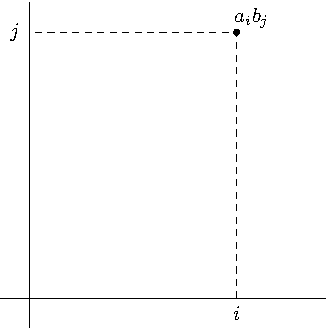
\includegraphics{images/cauchy1}
  \end{minipage}%
  \begin{minipage}{0.50\textwidth}
    \centering
    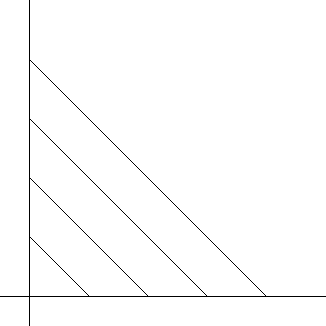
\includegraphics{images/cauchy2}
  \end{minipage}%
  \caption{Das Cauchyprodukt}%
  \label{fig:cauchy}
\end{figure}

\begin{example}
  Sei 
  \[
    a_k = b_k = {(-1)}^k \frac{1}{\sqrt{k+1}}.
  \]
  Die Reihe
  \[
    \sum_{k=0}^{\infty} {(-1)}^k \frac{1}{\sqrt{k+1}}
  \]
  konvergiert (nach dem Leibnizkriterium),
  da die Folge ${(1/\sqrt{k+1})}_{k \in \mathbb{N}}$
  monoton fallend ist mit Grenzwert null.
  Wir bestimmen nun den Summanden $c_n$ im
  Cauchyprodukt
  $\left( \sum_{i=0}^{\infty} a_i \right) \cdot
  \left( \sum_{j=0}^{\infty} b_j \right)$.
  Berechne
  \begin{align*}
    c_n & = \sum_{k=0}^{n} {(-1)}^k \frac{1}{\sqrt{k+1}}
    \cdot {(-1)}^{n-k} \cdot \frac{1}{\sqrt{n-k+1}} \\
        &=
    (-1)^n \left(  
      \frac{1}{\sqrt 1} \cdot \frac{1}{\sqrt{n+1}}
      + \frac{1}{\sqrt 2} \cdot \frac{1}{\sqrt n}
      + \frac{1}{\sqrt 3} \cdot \frac{1}{\sqrt{n-1}}
      + \cdots
      + \frac{1}{\sqrt{n+1}} \cdot \frac{1}{\sqrt 1}
    \right).
  \end{align*}
Jeder dieser $n + 1$ Summanden in $c_n$ ist grösser oder
gleich $1/(n+1)$, denn
\[
  \frac{1}{\sqrt{k+1}}\cdot\frac{1}{\sqrt{n-k+1}}
  \geq \frac{1}{\sqrt{n+1}} \cdot \frac{1}{\sqrt{n+1}}
  = \frac{1}{n+1}.
\]
Also ist $|c_n| \geq 1$ für alle $n \in \mathbb{N}$.
Insbesondere ist ${(c_{n})}_{n \in \mathbb{N}}$ 
keine Nullfolge,
also $\sum_{n=0}^{\infty} c_n$ nicht konvergent.
\end{example}

\begin{theorem}\label{thm:cauchy-product}
  Seien
  $\sum_{i=0}^{\infty} a_i$ und $\sum_{j=0}^{\infty} b_j$ 
  absolut konvergent mit Grenzwerten $\alpha$ und $\beta$ 
  in~$\mathbb{R}$.
  Dann konvergiert das Cauchyprodukt
  $\left( \sum_{i=0}^{\infty} a_i \right) \cdot
  \left( \sum_{j=0}^{\infty} b_j \right)$ mit
  Grenzwert $\alpha \cdot \beta$.
\end{theorem}

% \begin{proof}
%   Sei $N \in 2\mathbb{N}$ beliebig.
%   Setze
%    \[
%      A = \sum_{i=0}^{\infty} |a_i|, \;\; 
%      B = \sum_{j=0}^{\infty} |b_j|.
%    \]
%    Beachte, dass $A$ nicht unbedingt dasselbe
%    wie $\alpha$ und $B$ nicht unbedingt dasselbe
%    wie $\beta$ ist.
%    Wir behaupten, dass
%    \begin{align*}
%      \sum_{n=N}^{\infty} |c_n| & \leq
%      \left( \sum_{i=N/2}^{\infty} |a_i| \right)
%      \cdot
%      \left( \sum_{j=N}^{\infty} |b_j| \right)
%      +
%      \left( \sum_{i=0}^{\infty} |a_i| \right)
%      \cdot
%      \left(
%      \sum_{j=N/2}^{\infty} |b_j|\right),\\
%    \end{align*}
%    siehe Abbildung~\ref{fig:cauchy-proof}.
%    Es folgt, dass
%    $\sum_{n=N}^{\infty} |c_n| \leq
%    \left( \sum_{i=N/2}^{\infty} |a_i \right) \cdot B
%    + A \cdot
%    \left( \sum_{j=N/2}^{\infty} |b_j| \right).$
%    Aber das zeigt, dass
%    \[
%      \lim_{N \to \infty} \sum_{n=N}^{\infty} |c_n| = 0,
%    \]
%    da
%    \[
%      \lim_{n \to \infty} \sum_{i=N/2}^{\infty} |a_i| =
%      \lim_{n \to \infty} \sum_{j=N/2}^{\infty} |b_j| = 0.
%    \]
%    Also ist die Reihe $\sum_{n=0}^{\infty} c_n$ absolut
%    konvergent.

%    Zu zeigen bleibt, dass $\sum_{n=0}^{\infty} c_n = \alpha
%    \cdot \beta$. Man kann mit einem ähnlichen Argument
%    zeigen, dass
%    \[
%      \lim_{N \to \infty}
%      \left| 
%        \sum_{n=0}^{N} c_n -
%        \left( \sum_{i=0}^{N} a_i \right)
%        \cdot
%        \left( \sum_{j=0}^{N} b_j \right)
%      \right| = 0. \qedhere
%    \]
% \end{proof}

\begin{proof}
  Setze
  \[
    A = \sum_{i=0}^{\infty} |a_i| \text{ und }
    B = \sum_{j=0}^{\infty} |b_j|.
  \]
  Diese Grenzwerte existieren, da die beiden Reihen
  $\sum_{i=0}^{\infty} a_i$ und $\sum_{j=0}^{\infty} b_j$ 
  absolut konvergieren. Im allgemeinen stimmen $A$ und $B$
  aber nicht mit $\alpha$ und $\beta$ überein.
  Sei $N \in \mathbb{N}$. Wir schätzen ab:
  \begin{align*}
    \sum_{n=0}^{N} |c_n| &
    \leq \left(\sum_{i=0}^{N} |a_i|\right)
    \cdot \left( \sum_{j=0}^{N} |b_j| \right) \leq A \cdot B
  \end{align*}
  wobei
  \[
    c_n = \sum_{k=0}^{n} a_k b_{n-k}.
  \]
  In Abbildung~\ref{fig:cauchy-proof}
  sind die Terme links alle
  Punkte unter der
  gestrichelten Linie.
  Also ist die Reihe $\sum_{n=0}^{\infty} c_n$ absolut
  konvergent.

  Zu zeigen bleibt, dass der Grenzwert der Reihe
  $\sum_{n=0}^{\infty} c_n$ gerade $\alpha \cdot \beta$ 
  ist. Berechne dazu
  \begin{align*}
    \left| \left( \sum_{i=0}^{N} a_i \right)
    \left( \sum_{j=0}^{N} b_j \right) - \sum_{n=0}^{N} c_n \right| 
    & \leq \left(\sum_{i=N/2}^{\infty} |a_i| \right)
     \left( \sum_{j=0}^{\infty} |b_j| \right)
     + \left( \sum_{i=0}^{\infty} |a_i| \right)
     \left( \sum_{j=N/2}^{\infty} |b_j| \right)\\
    &= \left( \sum_{i=N/2}^{\infty} |a_i| \right) B
    + A \left( \sum_{j=N/2}^{\infty} |b_j| \right),
  \end{align*}
  siehe Abbildung~\ref{fig:cauchy-proof}: die
  Terme rechts von der Ungleichung sind alle Punkte
  im grau markierten Bereich,
  und die Terme links von der Ungleichung
  sind alle Punkte im vollständig grauen Dreieck.
  Aber
  \[
    \lim_{N \to \infty} \sum_{i=N/2}^{\infty} |a_i| = 0
    \text{ und }
    \lim_{N \to \infty} \sum_{j=N/2}^{\infty} |b_j| = 0,
  \]
  also gilt
  \begin{align*}
    \sum_{n=0}^{\infty} c_n 
    & = \lim_{N \to \infty} \sum_{n=0}^{N} c_n \\
    & = \left( \lim_{N \to \infty}\sum_{i=0}^{N} a_i \right)
    \left( \lim_{N \to \infty}\sum_{j=0}^{N} b_j \right) \\
    & = \alpha \cdot \beta. && \qedhere
  \end{align*}
\end{proof}


\begin{figure}[htb]
  \centering
  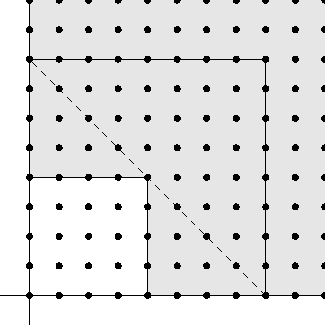
\includegraphics{images/cauchy-thm}
  \caption{Beweis der Konvergenz des Cauchyprodukts}%
  \label{fig:cauchy-proof}
\end{figure}

\newpage
\section{Die Exponentialfunktion}
\begin{lemma*}
  Sei $x \in \mathbb{R}$. Dann ist die Reihe
  $\sum_{k=0}^{\infty} \frac{x^k}{k!}$ absolut konvergent.
\end{lemma*}

\begin{proof}
  Sei zunächst $x \geq 0$. Wähle $N \in \mathbb{N}$ mit
  $N+ 1 \geq 2x$.
  Dann gilt für alle $n > N$, dass
  \begin{align*}
    \sum_{k=0}^{n} \frac{x^k}{k!}    & 
    = 1 + \frac{x}{1!} + \frac{x^2}{2!} + \cdots
    + \frac{x^N}{N!} + \cdots \frac{x^n}{n!} \\ &
    = 1 + \cdots + \frac{x^N}{N!}
    \left( 1 + \frac{x}{N+1} + \frac{x^2}{(N+1)(N+2)}
  + \cdots + \frac{x^{n-N}}{(N+1) \cdots n}\right)\\ &
    \leq 1 + x + \cdots \frac{x^{N-1}}{(N-1)!} + 2 \cdot
    \frac{x^N}{N!},
  \end{align*}
  da
  \begin{itemize}
    \item $x/(N+1) \leq 1/2$,
    \item $x^2/(N+1)(N+2) \leq 1/4$,
    \item $x^3/(N+1)(N+2)(N+3) \leq 1/8$,
  \end{itemize}
  und so weiter.
  Also ist die Folge der Partialsummen
  \[
    s_n(x) = \sum_{k=0}^{n} \frac{x^k}{k!}
  \]
  nach oben beschränkt und monoton wachsend, da $x \geq 0$.
  Folglich ist die Reihe
  $\sum_{k=0}^{\infty} \frac{x^k}{k!}$ absolut konvergent.
  Für $x < 0$ bemerken wir,
  dass die Reihe
  \[
    \sum_{k=0}^{\infty} \left| \frac{x^k}{k!} \right|
    = \sum_{k=0}^{\infty} \frac{|x|^k}{k!}
  \]
  konvergiert (siehe oben), also auch die Reihe
  $\sum_{k=0}^{\infty} x^k/k!$.%chktex 40
\end{proof}

\begin{definition}
  Die \emph{Exponentialfunktion} ist die Funktion
  \begin{align*}
    \exp \colon \mathbb{R} & \to \mathbb{R} \\
    x & \mapsto \sum_{k=0}^{\infty} \frac{x^k}{k!}.
  \end{align*}
\end{definition}

\begin{theorem}\label{thm:exp-product-sum}
  Für alle $x, y \in \mathbb{R}$ gilt
  \(
    \exp(x + y) = \exp (x) \cdot \exp (y).
  \)
\end{theorem}

\begin{proof}
  Berechne das Cauchyprodukt
  der beiden absolut konvergenten Reihen
  $\exp(x)$ und $\exp(y)$ wie folgt:
  \begin{align*}
    \exp(x) \cdot \exp(y) & =
    \left(\sum_{i=0}^{\infty} \frac{x^i}{i!}\right)
    \left( \sum_{j=0}^{\infty} \frac{y^j}{j!} \right)\\ &
    = \sum_{n=0}^{\infty} \sum_{k=0}^{n} \frac{x^k}{k!} 
    \frac{y^{n-k}}{(n-k)!} \\ &
    = \sum_{n=0}^{\infty} \frac{{(x + y)}^n}{n!} \\&
    = \exp(x + y)
  \end{align*}
  nach Theorem~\ref{thm:cauchy-product},
  da
  \[
    {(x + y)}^n = \sum_{k=0}^{n} \frac{n!}{k! {(n-k)}!} x^k y^{n-k}.
    \qedhere
  \]
\end{proof}

\begin{eig-exp}
  \leavevmode
  \begin{enumerate}[\normalfont(i)]
    \item $\exp(0) = 1$ und $\exp(1) = e$, die Eulersche Zahl
      (siehe Serie 4).
    \item Für $h \geq 0$ gilt $\exp(h) \geq 1 + h$,
      und für $0 \leq h \leq 1$ gilt  
      \[
        1 + h \leq \exp(h) \leq 1 + 2h,
      \]
      (siehe Serie 4). %TODO check.
    \item Für alle $x \in \mathbb{R}$ gilt
      \(
        \exp(-x) = {1}/{\exp(x)}.
      \)
      Dazu berechne
      \[
        \exp(0) = \exp(x - x) = \exp(x) \cdot \exp(-x)
      \]
      nach Theorem~\ref{thm:exp-product-sum}.
    \item Für alle
      $n \in \mathbb{N}$ gilt $\exp(n) = e^n$. Berechne dazu
      \[
        \exp(n) = \exp(1 + \cdots + 1) =
        {\left( \exp(1) \right)}^n = e^n.
      \]
  \end{enumerate}
\end{eig-exp}

\begin{notation}
  Wir schreiben von nun an auch
  \(
    e^x = \exp(x).
  \)
\end{notation}

\begin{proposition*}
  Die Exponentialfunktion $\exp \colon \mathbb{R} \to \mathbb{R}$ 
  ist positiv, streng monoton wachsend, und surjektiv
  als Funktion $\mathbb{R} \to \mathbb{R}_{>0}$.
\end{proposition*}

\begin{proof}
  \leavevmode
  \begin{itemize}
    \item \emph{Positivität}. 
      Für $x \geq 0$ gilt $\exp(x) \geq 1$,
      und für $x < 0 $ gilt $\exp(x) = 1/\exp(-x)$
      (siehe Eigenschaft (iii)), also gilt
      auch in diesem Fall
      $\exp(x) > 0$.
    \item \emph{Monotonie}. 
      Seien $x, y \in \mathbb{R}$ mit $x < y$.
      Dann gilt:
      \[
        \exp(y) = \exp(x + (y - x))
        = \exp(x) \cdot \exp(y-x)
        > \exp(x),
      \]
      da $\exp(y-x) > 1$.
    \item \emph{Surjektivität}.
      Sei $y > 0$. Wir behaupten,
      dass $x_1, x_2 \in \mathbb{R}$ existieren mit 
      \[
        \exp(x_1) < y < \exp(x_2).
      \]
      Setze dazu $x_2 = y$. Dann ist
        $\exp(x_2) \geq 1 + y > y$.
      Für $x_1$ machen wir eine Fallunterscheidung.
      Falls $y > 1$, setze $x_1 = 0$. Dann ist
      $\exp(x_1) = 1 < y$. Für $y \leq 1$, setze
      $x = -1/y$. Dann ist
       \[
         \exp(x_1) = \frac{1}{\exp(1/y)} < \frac{1}{1/y} = y.
      \]
      Dies zeigt die Behauptung, dass wir jeden gewünschten
      Wert überbieten und auch unterbieten können.

      Zu zeigen bleibt, dass wir den gewünschten Wert auch
      tatsächlich treffen.
      Wir suchen also $s \in \mathbb{R}$ mit $\exp(s) = y$.
      Wir konstruieren dieses $s$ mit dem Supremumsprinzip.
      Definiere
      $A = \left\{x \in \mathbb{R} \mid \exp(x) \leq y\right\}$,
      siehe Abbildung~\ref{fig:exp}.
      Nach obiger Behauptung ist $A$ nicht leer,
      da $x_1$ existiert mit $\exp(x_1) \leq y$.
      Weiter ist $A$ nach oben beschränkt,
      da $y \leq \exp(x_2)$.
      Setze nun $s = \sup(A) \in \mathbb{R}$.
      Wir zeigen, dass $\exp(s) = y$ indem wir
      beide Ungleichungen zeigen.

      Nehme widerspruchsweise an, dass $\exp(s) < y$.
      Wähle $h \in \mathbb{R}$ mit $0 < h < 1$
      und $1 + 2h \leq y/\exp(s)$.
      Dies funktioniert, da $y/\exp(s) > 1$.
      Es gilt dann
       \[
         \exp(s + h) = \exp(s) \cdot \exp(h) \leq \exp(s)
         \cdot (1 + 2h) \leq y
      \]
      nach Eigenschaft (ii).
      Also ist $s + h \in A$, was im Widerspruch zu
      $s = \sup(A)$ steht.
      Somit folgt $\exp(s) \geq y$.
      
      Umgekehrt, nehme widerspruchsweise an,
      dass $\exp(s) > y$. Ähnlich wie im ersten Schritt, wähle
      $h \in \mathbb{R}$ mit $0 < h \leq 1$ 
      und $1 + 2h \leq \exp(s)/y$.
      Dann gilt
      \[
        \exp(s-h) = \frac{\exp(s)}{\exp(h)}
        \geq \frac{\exp(s)}{1 + 2h} \geq y.
      \]
      Also ist $s-h$ eine obere Schranke für $A$,
      im Widerspruch dazu dass $s = \sup(A)$ die
      kleinste obere Schranke für $A$ ist.
      Folglich gilt $\exp(s) \leq y$. \qedhere
  \end{itemize}
\end{proof}

\begin{figure}[htb]
  \centering
  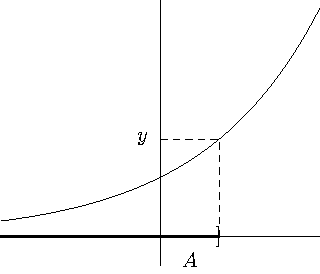
\includegraphics{images/exp}
  \caption{Beweis der Surjektivität der Exponentialfunktion}%
  \label{fig:exp}
\end{figure}


\begin{remark}
  Die Menge $\exp(\mathbb{Q})$ ist nicht die Menge
  $\mathbb{Q}_{>0}$ der positiven rationalen Zahlen.
  Tatsächlich ist das Bild der meisten rationalen Zahlen
  nicht rational (das ist schwierig zu zeigen).
  Der Satz oben funktioniert also nur über $\mathbb{R}$.
\end{remark}

\subsection*{Der Logarithmus}
Wir wissen, dass die Exponentialfunktion
$
  \exp \colon \mathbb{R} \to \mathbb{R}_{>0}
  $
streng monoton wachsend und surjektiv ist.
Insbesondere ist $\exp$ bijektiv.

\begin{definition}
  Die \emph{Logarithmusfunktion}
  $\log \colon \mathbb{R}_{>0} \to \mathbb{R}$ ist die
  eindeutige Umkehrfunktion der Exponentialfunktion,
  das heisst $\log = \exp^{-1}$.
\end{definition}

\begin{remark}
Es gilt für alle $a, b > 0$, dass
\[
  \log(a \cdot b) = \log(a) + \log(b).
\]
Dazu bemerke, dass
\[
  \exp(\log(a) + \log(b)) = 
  \exp(\log(a)) \cdot \exp(\log(b))
  = a \cdot b = \exp(\log(a \cdot b)).
\]
Da die Exponentialfunktion injektiv ist,
folgt die Behauptung.
\end{remark}

\begin{definition}
  Sei $a > 0$ und $x \in \mathbb{R}$. Wir definieren
  die allgemeine \emph{Potenzfunktion}
  $x \mapsto a^x$ durch
  \[
    a^x = \exp(\log(a) \cdot x).
  \]
\end{definition}

\begin{remark}
  Für alle $x, y \in \mathbb{R}$ gilt
  \[
    a^{x+y} = a^{x} \cdot a^{y}.
  \]
\end{remark}
\end{document}

